% Chris Cornwell, Ian M. Schmutte, Daniela Scur
% v1.0 
% Last updated, 5 Aug 18

%%%%%%%%%%%%%%%%%%%%%%%%%%%%%%%%%%%%%%%
\documentclass[12pt]{article}
%TCIDATA{OutputFilter=Latex.dll}

	%TCIDATA{LaTeXparent=0,0,noname.tex}

%-------------------- Packages --------------------
    \usepackage{booktabs}
    \usepackage{epstopdf}
	\usepackage{fancyref}
	\usepackage{array}
	\usepackage{hyperref}
	\usepackage{graphics}
	\usepackage{float}
	\usepackage{subcaption}
	\usepackage{caption}
	\usepackage{amsfonts}
	\usepackage{amsmath}
	\usepackage{natbib}    % for bibliography
	\usepackage{amssymb}  % AMS symbols
	\usepackage{amsfonts}
	\usepackage{tikz}		%for nice-looking graphs
	\usepackage{pgfplots}	%for nice-looking plots of data (requires tikz package)
		\pgfplotsset{compat = newest} %to use newest plot settings in pgfplot
	\usepackage{graphicx} % for inclusion of EPS graphics
	\usepackage{multicol} % Multicolumn formatting (in-line tables)
	\usepackage{rotating}  % allows for rotated tables
	\usepackage{setspace}
	\usepackage{multirow} %allows multirows/cols in tabls
	\usepackage{array}     % Modifications of tabular environment
	\usepackage{threeparttable} %Allows tables with automatic notes section
	\usepackage{longtable} % allows for tables to wrap across pages.
	\usepackage{supertabular} % allows for tables to wrap across pages.
	% \usepackage{subfloat}	%to put multiple floats in the same frame
	\usepackage{color}
	\usepackage{lscape}
	\usepackage{geometry}
	%\makeindex
	\usepackage{dcolumn}
	\newcolumntype{k}{D{.}{.}{1.3}}
	\newcolumntype{d}{D{.}{.}{2.2}}
	\newcolumntype{s}{D{.}{.}{1.0}}
	\newcommand{\m}[1]{\multicolumn{1}{c}{#1}} %for use with dcolumn
	\newcolumntype{f}{D{.}{.}{2.4}}

%-------------------- hyperref setup-----------------
	% defining colors for package hyperref
	\definecolor{myblue}{rgb}{0,.2,1}

	\hypersetup{%
	%backref=true,%
	naturalnames=true,%
	bookmarksnumbered=true,%
	bookmarksopen=false,%
	plainpages=true,%
	colorlinks=true,%
	urlcolor=myblue,
	linkcolor=myblue,%
	filecolor=myblue,%
	citecolor=black,%
	%pagecolor=myblue,%
	%pdftitle={\myshorttitle},%
	%pdfpagemode=UseOutlines,%
	%pdfauthor={\myshortauthors},%
	%pdfsubject={\myshorttitle}
	}%

%----------------------
	%To insert un-numbered footnotes (as on the title page)
	%ref: http://en.wikibooks.org/wiki/LaTeX/Formatting#cite_note-csli_footnotes-0
	\makeatletter
	    \def\blfootnote{\xdef\@thefnmark{}\@footnotetext}
	\makeatother
	% http://tex.stackexchange.com/questions/8351/what-do-makeatletter-and-makeatother-do


%-------------------- choose the font here --------------------
	\usepackage{times}
	%\usepackage{newcent}
	%\usepackage{helvet}
	%\usepackage{helvetic}
	%\usepackage{ncntrsbk}
	%\usepackage{bookman}
	%\usepackage{avantgar}
	% \usepackage{palatino}

%-------------------- formatting of fancy references --------------------
	%\newcommand{\Cite}{\citeasnoun} % this for harvard
	\newcommand{\Cite}{\citet} % this for natbib
	\bibpunct{(}{)}{;}{a}{}{;} %set if using natbib

%-------------------- Common Math Operators ----------
	\DeclareMathOperator{\Corr}{Corr}
	\DeclareMathOperator{\cov}{cov}
	\DeclareMathOperator{\var}{var}
	\DeclareMathOperator{\E}{E}
	\DeclareMathOperator{\F}{F}
	\DeclareMathOperator{\f}{f}
	\DeclareMathOperator{\J}{J}
	\DeclareMathOperator{\Tp}{T}

%-------------------- Special Commands
	\newcommand{\s}{^{*}} %for putting stars in tables
	\renewcommand{\ss}{^{**}}
	\newcommand{\sss}{^{***}}
	\newcommand{\fnone}{\textsuperscript{1}}
	\newcommand{\fna}{\textsuperscript{a}}
	\newcommand{\fnb}{\textsuperscript{b}}
	\newcommand\T{\rule{0pt}{2.6ex}}         %for manipulating space in tables
	\newcommand\B{\rule[-1.2ex]{0pt}{0pt}}	 %for manipulating space in tables
	\newcommand\C{\rule{0pt}{0pt}}
	\newcommand\mrt{\multirow{2}{*}}

%-------------------- Common Theorem Environments ------------------------
	\newtheorem{theorem}{Theorem}
	\newtheorem{algorithm}{Algorithm}
	\newtheorem{axiom}{Axiom}
	\newtheorem{case}{Case}
	\newtheorem{claim}{Claim}
	\newtheorem{conclusion}{Conclusion}
	\newtheorem{condition}{Condition}
	\newtheorem{conjecture}{Conjecture}
	\newtheorem{corollary}{Corollary}
	\newtheorem{criterion}{Criterion}
	\newtheorem{definition}{Definition}
	\newtheorem{example}{Example}
	\newtheorem{exercise}{Exercise}
	\newtheorem{lemma}{Lemma}
	\newtheorem{notation}{Notation}
	\newtheorem{problem}{Problem}
	\newtheorem{proposition}{Proposition}
	\newtheorem{remark}{Remark}
	\newtheorem{solution}{Solution}
	\newtheorem{summary}{Summary}




%%% End:  %packages, special commands, environments defined here
	% \input{./tcilatex} %pulls in TCILATEX macros in case someone used SciWord.

%------------- Edit at your own risk ---
%%%%%%%%%%%%%%%%%%%%%%%%%%%%%%%%%%%%%%%%
\pagestyle{plain}                     %%
%%%%%%%% EXACT 1in MARGINS %%%%%%%%%%%%%
\setlength{\textwidth}{6.5in}     %%  %%
\setlength{\oddsidemargin}{0in}   %%  %%
\setlength{\evensidemargin}{0in}  %%  %%
\setlength{\textheight}{8.75in}   %%  %%
\setlength{\topmargin}{0in}       %%  %%
\setlength{\headheight}{0in}      %%  %%
\setlength{\headsep}{0in}         %%  %%
\setlength{\footskip}{.5in}       %%  %%
%%%%%%%%%%%%%%%%%%%%%%%%%%%%%%%%%%%%%%%%
%%%%%%%%%%%%%%%%%%%%%%%%%%%%%%%%%%%%%%%%

%-------------------- Special Commands-------------------------------
	%to make the table numbering with Roman numerals
	\renewcommand{\thetable}{\Roman{table}}

	%try to eliminate the stupid * for \thanks in titlepage
	\renewcommand\footnotemark{}

%-------------------- Document information---------------------------
	\newcommand{\mytitle}{How Structured Personnel Management Practices Lead to a Productive Workforce}
	\newcommand{\myshorttitle}{Structure management practices}
	\newcommand{\myshortauthors}{Cornwell, Schmutte, and Scur}
	\newcommand{\myauthors}{Chris M.\ Cornwell \and Ian M.\ Schmutte \and Daniela Scur}
	\newcommand{\myversion}{\today}
	\newcommand{\RAISDisclaimer}{
		}
	\newcommand{\mythanks}{\noindent We use the Brazilian employer-employee dataset (RAIS) data under an agreement with the \emph{Minist\'{e}rio do Trabalho e Emprego} (MTE), Brazil's labor ministry, which collects and maintains RAIS. We thank Carlos Lessa at the Brazilian statistics agency (IBGE) for access to the Brazilian industrial survey data (PIA). We thank participants at the LERA Session at ASSA 2017 and the Empirical Management Conference 2018 for useful discussions and comments. %
		}
%LERA Session at ASSA 2017, Ekaterina Roshchina, Lisa Kahn, Christos Makridis, Nick Bloom, John van Reenen, Rafaella Sandun

%--------------------------------------------------------------------

% Daniela's packages - feel free to edit if need be or if it screws anything up

% Ensuring the accents are added
\usepackage[T1]{fontenc}
\usepackage[utf8]{inputenc}

% Making the links blue - personal choice, happy to change it if people don't like it!
\hypersetup{
	colorlinks=true,
	linkcolor=black,
	anchorcolor=black,
	citecolor=blue,
	urlcolor=blue
}

\usepackage{pdflscape}

%%%%%%%%%%%%%%%%%%%%%%%%%%%%%%%%%%%%%%%%%%%%%%%%%%%%%%%%%%%%%%%%%%%%%
%%%%%%%%%%%%%%%%%%%%%%%%%%%%%%%%%%%%%%%%%%%%%%%%%%%%%%%%%%%%%%%%%%%%%

\begin{document}

% section section_name (end)

%%%%%%%%%%%%
%Title Page
%%%%%%%%%%%%
    \makeatletter
	\begin{titlepage}
		\begin{center}
			\MakeUppercase{\mytitle} \\ [2cm]
			\begin{tabular}{c@{\hskip .25in}c@{\hskip .25in}c}
			Christopher Cornwell   	  & Ian M.\ Schmutte 		  & Daniela Scur			   \\
			Department of Economics   & Department of Economics   & Sloan School of Management \\
			Terry College of Business & Terry College of Business & MIT        				   \\
			University of Georgia 	  & University of Georgia 	  & dscur@mit.edu              \\
			cornwl@uga.edu			  & schmutte@uga.edu          &                            \\
			\end{tabular} \\ [1cm]
			\myversion \blfootnote{\mythanks} \\  [1cm]
		\end{center}

		\singlespacing
		\small
		\noindent It is well established that organizational practices matter for workforce composition and productivity, but the mechanisms behind these effects are less well understood. In this paper, we explore how structured personnel management practices relate to actual HR outcomes and productivity. We match structured management practices data from the World Management Survey to AKM estimates of worker and firm fixed effects and industrial survey data from ten years of Brazilian  administrative data. We have four key findings: first, consistent with the literature, we find that worker and manager fixed effects, as well as structured management, are positively correlated with firm productivity. Second, we find evidence of positive recruitment: better managed firms hire a larger share of their new recruits --- managers and production workers --- from the top of the distribution of worker fixed effects. Third, we find suggestive evidence of better worker matching and retention from lower separation rates. Fourth, we decompose the variation of personnel management practices and find that promotion and retention practices show the strongest correlation with manager fixed effects. 
	\end{titlepage}
	% \makeatother
	% \maketitle

	% ------------------------------ Main Document Body-----------------
    \onehalfspacing 
    \section{Introduction} 
    \label{sec:introduction}
    % !TeX root = ./AER_Insights.tex

This paper studies the role of management in assembling a high quality and productive workforce. On this topic, existing empirical research provides two different kinds of evidence, the first based on surveys about the practices of plant managers, and the second based on the observed hiring, firing, and compensation outcomes of individual firms. 
In the World Management Survey, for example, managers report whether they have formal practices in place to attract and retain skilled workers, to create incentives for high-performing workers, and for identifying and removing their less effective employees \citep{Bloom2012}. 
By contrast, most studies based on observational data do not know about the practices used by management, and instead study patterns in data on pay and job transitions to infer the nature of decision-making within the firm \citep[e.g.][]{AbowdKramarzRoux:EJ:2006,Hensvik2018}.
It is natural to surmise that the inferred behaviors drawn from observational data reflect the implementation of formal management practices described in the survey-based literature. This need not be the case. Many models of the labor market illustrate that different firms may optimally attract workers of differing ability, without reference to specialized investments in managerial processes, nor in managerial talent.\footnote{The assortative matching model of \citet{becker1973theory} is the classic example, but in most contemporary discussions of job matching in economics, like \citet{Card:FirmsIneq:JOLE:2017} or \citet{Sorkin:Ranking:QJE:2018}, matching happens without the intervention of any particular or specialized managerial competence.} It is clear that labor market models abstract away from real-world differences in the personnel management practices of different firms. It is less clear how much those differences matter, and why.

We combine the approaches in the prior literature to assess the relationship between a firm's stated use of what we call \emph{structured} management practices and its observed success in hiring and retaining high-quality workers. Despite a large conceptual and theoretical body of work on ``what managers do'' \citep{gibbonshenderson_2012}, there is still little empirical evidence on how the practices employed by managers affect workforce quality. Structured management practices must be implemented by skilled managers, %insert citation
 and so we focus in particular on the quality of both the managerial and non-managerial workforce. We find that firms using structured management practices are indeed more successful, both at recruiting and keeping better managers, as well as better production workers. We also provide evidence that these findings reflect behavioral differences between firms that use structured management practices and those that do not.

Our analysis is based on a unique dataset that links firm-level survey measures of management practices from the World Management Survey (WMS) to matched employer-employee data from Brazil, the \emph{Rela\c{c}\~{a}o Anual de Informa\c{c}\~{o}es Sociais} (RAIS). The WMS data provide consistent measures of the management practices in a representative repeated cross-section of manufacturing establishments in Brazil (along with thirty-four other countries, \citet{bloom_qje2007}. 
% The WMS interview covers 18 basic management practices, a third of which relate specifically to the ``people'' or personnel management practices that directly target hiring, retention and dismissal decisions. 
Based on these data, we characterize each firm as having either structured or unstructured management practices, with respect to both its management of people, and its management of production operations. We match these management statistics to a specific measure of the quality of each establishment's managerial and non-managerial workforce derived from the RAIS. The longitudinal structure of RAIS lets us measure each firm's success in using hiring, firing, and retention to maintain a high-quality workforce.

%In Section \ref{}, we introduce our data and describe how we measure our key concepts, namely structured management practices, and worker quality. There, we also describe how we use establishment-level productivity data to validate our measure of worker quality. In Section \ref{}, we present our main findings. 
Our findings can be summarized as follows. First, firms with structured personnel management practices hire disproportionately from the top half of the worker quality distribution, especially when recruiting managers. Second, these firms are also more successful at keeping their high-quality hires. Their incumbent managers are twice as likely to be high-quality and their advantage among incumbent production workers is almost as great. Third, firms with structured management practices have much lower overall rates of quits and fires, suggesting they screen or motivate workers more effectively. Furthermore, when they do dismiss workers, firms using structure practices fire more selectively with respect to worker quality.  Finally, we show that the most important personnel practice for attracting and retaining a high-quality workforce is ``instilling a talent mindset'', where hiring high-quality workers is expressly a top priority for the firm and senior managers are rewarded accordingly.  This is true for both production workers and managers. However, we also find that operations management practices are relatively more important for explaining variation in manager quality, suggesting that well-defined targets, accountability and performance evaluation facilitate matches with better managerial talent. 

The key takeaway is that the way workers match to firms depends on the quality of each firm's management practices and the allocation of managerial talent. Our results thus speak to a need for further integration between research on the role of firms in labor markets and research on organizational behavior focused on recruiting and retention. A handful of other papers have arrived at similar conclusions. Similar to our paper, \citet{Bender:Management:JOLE:2018} document a positive relationship between firm productivity and worker quality using WMS data linked to German administrative records. Unlike them, we are able to distinguish managerial workers directly, and can isolate the different interactions between management practices and managerial versus non-managerial workers.
\citet{Bandiera:Matching:JOLE:2015} use Italian administrative data to explore how managers and firms match through high- and low-powered incentives.  Finally \citet{Hoffman:Discretion:QJE:2018} shows that good management practices are needed to overcoming managerial biases in hiring decisions.

Taken together, the literature suggests that the institutional environment in the firm, manifest in its management practices, cannot be reduced to the quality of its managers or its workforce. 
The labor literature highlights the importance of firms and worker-firm matching for understanding inequality \citep{Card2013,Alvarez:Firms:AEJM:2018,Song:Firming:QJE:2018}, gender wage gaps \citep{Card:Bargaining:QJE:2016}, compensating differentials \citep{Lavetti:CDEM:WP:2018,Sorkin:Ranking:QJE:2018}, and productivity \citep{Iranzo2008}. 
These findings suggest that firms' decisions about who to hire and fire affect not only their own bottom line, but the functioning of the entire labor market. 
However, these studies generally abstract away from the processes firms use to assemble their workforce.
\citet{OyerSchaefer:HLE:2011}, suggest that economists should focus on the active role played by management in recruiting the best workers. Recent research based on observational data points to the importance of good managers for team production \citep{shaw_bosses,Hensvik2018}, managing the cost of turnover \citep{Jager2016,Gallen2018}, and
the selection of skilled workers \citep{Friedrich2017}. 
Therefore, understanding how firms interact with and affect labor markets can and should be further investigated as data on management practices and linked employer-employee data become more widely available.




 

% However, each of these papers lacks some important element of our unique empirical setting -- either the ability to distinguish managers from production workers, identify the reason for separation or empirically measure managerial practices.



% Eeckhout and Kircher (2011) 
	
	\section{Empirical Setting} 
	\label{sec:setting}
	% Last updated:
% 10 Apr 2019, CC
%!TEX root=MGMT.tex

The empirical setting for our analysis combines three datasets covering Brazilian firms: RAIS, which provides essential information on workers and their jobs; the WMS, which contributes our measures of management practices; and Annual Industrial Survey (\textit{Pesquisa Industrial Anual - PIA}), our source for firm input and output data.

\subsection{Occupation, employment history and worker quality: RAIS}
% 1. What RAIS provides
For every formal sector job, RAIS reports the employee's monthly earnings, occupation, hours of work, education, gender and race, along with the firm's industry and municipality. With the occupation data, we are able to distinguish managers from production workers. Importantly for our purposes, it also records the date of hire, month and year of separation, and reason for separation, and, for new hires, whether the job is their first registered employment.

%\subsubsection{Wage decomposition and worker quality}
%\label{sec:wage decomposition}

% 2. Worker-firm RAIS panel and worker quality
The RAIS data are also the basis for our measure of worker quality, which we define as the value of the skills a worker takes from job to job.  We isolate the contribution of these skills as the estimated worker effect from an AKM-style wage decomposition.  For the wage decomposition, we use the 2003-2013 waves and construct a sample of employees who are contracted to work at least 30 hours per week, have least one month of tenure and have complete set of covariates. We exclude workers in sole-proprietorships, establishments with only one employee, and observations beyond the top and bottom 0.01 percent of the wage distribution. These restrictions leave us with 353,141,951 unique worker-firm-year observations consisting of 96,499,697 unique workers and 4,433,492 unique establishments. Appendix \ref{app:EmpiricalDetails} provides details of the sample construction and summary statistics on the workers that comprise it.
% We need a cleaner mapping of this subsection to Appendix A and Table C.1.  Table C.1 does not literally provide summary statistics on the wage decomp variables as indicated in v1.1, e.g., experience is missing.  It is more an overview of the analysis sample, which is how it is described above.
% Workers are identified based upon their 16-digit PIS/PASEP numbers. As is standard, we restrict attention to the worker’s “dominant” job – their highest paying job during a given year.
% Need some new sentences to describe the multiple job possibilities in the current sample.
% NOTE - About 99% of people (PIS codes) are associated with 1 or 2 contracts per year (we have this in a SAS log). I'm just restricting analysis to cover all jobs for people with 2 jobs or less (along with the rest of our sample restrictions)
% *INSERT updated observation figures below.
% From CG_est_twfe_exp_normalized.log
% Starting Breadth-First Search to Count Components
% %%%%%%%%%%%%%%%%%%%%%%%%%%%%%%%%%%%%%%%%%%%%%%%%%
% Graph structure: I=96499697. J=4433492. Number of edges=161879895.
% Done finding connected components. Mopping up singletons.
% From 01.02.RAIS_prep_for_CG.lst
% % Number of observations: 353141951

% 3. Measuring worker quality
% !TeX root = ./AER Insights.tex
% Last updated:
% 11 Apr 19 - CC

Following \citet{Abowd1999}, the wage decomposition involves estimating a two-way, fixed-effects wage equation of the form
%
	\begin{equation}
	\label{eq:AKM_full}
	\ln y_{it} = \alpha + x_{it}\beta + \psi_{J(i,t)} + \theta_i 
	         + \varepsilon_{it},
	\end{equation}
where $y_{it}$ is the wage of worker $i$ at time $t$.\footnote{For the wage variable we take average monthly earnings, reported in 2003 Brazilian Reais, and convert it into an hourly measure. The monthly earnings data can be thought of as measuring the contracted monthly wage, a common institutional arrangement in Brazil. We convert this to an hourly measure by dividing the monthly wage by contracted hours per week, and then by 4.17. When a worker is employed for 12 months, average monthly earnings is simply annual earnings divided by 12. When a worker is employed fewer than 12 months, the total earnings paid for the year are divided by the number of months worked; for partial months, the earnings are pro-rated to reflect what the worker would have earned for the entire month. All of these calculations are performed by the MTE and included in the raw RAIS data.} In our specification, $x_{it}$ contains a cubic in labor-market experience interacted with race and gender.\footnote{For workers whose first employment begins in 2003 or after, experience is the sum of all months they are reported in at least one active employment relationship. For workers whose first employment started prior to 2003, we approximate experience as the greater of potential experience (age-years of schooling-6) or tenure in the first observed job.}   The $\psi_{J(i,t)}$ are firm effects that reflect employer-specific wage premia paid by establishment $j=J(i,t)$, where $J(i,t)$ indicates worker $i$'s job in year $t$ and $\varepsilon_{it}$ is a mean-zero error. Our primary interest is in the worker effects, $\theta_i$, which capture the value of portable skills and represent our measure of worker quality. Under strict exogeneity of $\varepsilon_{it}$ with respect to $x_{it}$, $\theta_i$ and $\psi_{J(i,t)}$, least squares will produce unbiased estimates of the worker and firm effects.\footnote{However, as explained in \citet{Abowd1999}, this assumption rules out endogenous mobility.} 

Similar to other settings --- for example, Germany \citep{Card2013}, Portugal \citep{Card:Bargaining:QJE:2016} and the US \citep{Abowd:EndMob:CES:2015} --- we find the AKM model provides a  thorough description of the sources of wage variation, with an $R^2$ above .90. Worker quality ($\hat\theta_i$) accounts for just under half of the total variation in log wages.  By contrast, the firm-specific component of pay ($\hat\psi_j$), explains $18.5$ percent. Table \ref{tab:AKM_vardecomp} and \ref{tab:AKM_corr} reports the canonical AKM variance decomposition and correlation tables.
 

% 4. Firm-level worker quality
We compute a firm-level worker-quality measure by averaging the estimated $\theta_i$ across worker occupations. In the WMS firms, roughly 5 percent of the employees hold managerial positions and the remaining 95 percent fill production jobs.\footnote{This is consistent with the WMS responses which indicate the average share of managers in a firm is 4.88 percent.} Average worker quality measures for managers in these firms is almost twenty times that of production workers.  However, manager quality is also more variable, with a standard deviation of 0.389 compared with 0.305 for production workers. Figure \ref{fig:pe_kdensity} compares compares the manager and production-worker quality distributions.

%see 01.01.analysis.log lines 93--96 10/26/2018
%     Variable |        Obs        Mean    Std. Dev.       Min        Max
% -------------+---------------------------------------------------------
%      pe_labr |        957    .0231546    .3046809  -.4973489   1.428571
%      pe_mngr |        953    .4064845    .3894263  -.4746531   2.733089

	
\subsection{Structured management practices: WMS}


% 1. Brief WMS overview
\subsubsection{Measuring management: the WMS survey methodology}
As described in \citet{bloom_qje2007}, the WMS project constructs measures of management practices from responses of senior plant managers on a set of 18 key practices. A third of these practices relate specifically to the ``people'' or personnel management practices that directly relate to hiring, retention and dismissal decisions. We follow (\citet{lemos_ej}) and group the other 12 practices, which concern lean operations, monitoring and target-setting, into a single operations index.  Responses are scored from 1 (``worst practice) to 5 (``best practice''), indicating the degree to which formal processes are in place. 
%a score of 1 indicates no formal or informal practices; 2 indicates some informal practices are in place; 3 indicates formal practices in place but with weaknesses; 4 indicates solid formal practices and 5 represents stable best practices. A high score implies that a firm has adopted a series of \textit{structured} management practices, which are associated with improvements in productivity \citep{bloom_india2012}.\footnote{See \citet{wms_jeea} for a survey.}
%A score of 3 and above indicates that there are some formal processes in place, while a score of 2 and below implies that only informal processes are in place, which are followed only if individual manager responsible for carrying them out is present. 
For example, consider the personnel practice of ``instilling a talent mindset'', which we find to be the most important for building a high-quality workforce.  Here, 1 implies that ``senior management does not communicate that attracting, retaining and developing talent throughout the organization is a top priority,'' while 5 means that ``senior managers are evaluated and held accountable on the strength of the talent pool they actively build.'' So, in this case, the ``best'' practice involves \textit{formal} accountability and performance evaluation processes \textit{structured} around a manager's contribution to workforce quality.

We use standardized averages of overall, personnel and operations practices in our analyses that call for continuous measures.\footnote{Specifically, we standardize each of the 18 questions, average over each index (overall, personnel and operations management) and standardize again.} For qualitative analyses, we follow the WMS scoring guide and distinguish between firms with at least some formal structures in place (scores of 3 or above) and those with none (scores of 2 or below). We use this conceptual divide to classify our firms as having ``structured practices'' (meaning \textit{formal processes}) or ``unstructured practices'' (meaning \textit{informal processes}). 

%Previous work with the WMS data has focused on using the standardized average of the 18 management practices scores, and we follow this convention in our regression analyses that focus on the continuous measure of structured management.\footnote{Specifically, we standardize each of the 18 questions, average across each index (overall management, operations and people management) and standardize again. We also follow the more recent convention (\citet{lemos_ej}) of grouping the 12 operations questions --- formally lean operations, monitoring and target setting questions --- and the 6 people management questions into two separate indices, rather than using four separate indices.} We use the average management practices score (all 18 topics), as well as a sub-index for only the ``people management'' questions (6 topics) and one for the ``non-people management'' questions (12 topics). In our figures, we depart from the data-driven approach to determining cut-offs and use a methodology-driven approach that focuses on the implicit meaning of the management scores when they were being awarded to firms during the data collection. In the WMS scoring guide, a score of 3 and above implies that there are at least some formal structures in place, while a score of 2 and below implies that while there may be a process in place, it is entirely informal and it would not be carried out if the individual manager who led it was not present. We use this conceptual divide to classify our sample into firms that have ``structured management'' (meaning \textit{formal processes}) and ``unstructured management'' (meaning \textit{informal processes}). We choose this nomenclature to avoid confusing informal processes with the informal sector, which is a large and important part of the Brazilian economy.

\subsubsection{Matched RAIS-WMS sample}

%Figures in first two pars should align with Table C.2. Table should collapse management indices to the two we use. 
There are 763 unique firms in the Brazilian sample of the WMS: 227 surveyed in 2008 only, 228 surveyed in 2013 only, and 308 surveyed in 2008 and 2013. Of the 763 firms, 694 can be matched to our RAIS sample for at least one year (213 in 2008, 214 in 2013 and 267 in both years), yielding 961 total observations between 2008 and 2013.\footnote{Employees are matched to their employers through a code assigned by the \textit{Cadastro Nacional da Pessoa Jur\'{i}dica} (CNPJ), which also allows a match to the WMS and PIA. Of the 763 WMS firms, 745 have valid CNPJ identifiers.} 

The average firm has 600 employees over than three production sites, with three layers between the CEO and shop floor. In the typical firm, only 13 percent of all workers have a university degree, while 73 percent of managers do. Over 75 percent of firms have at least five competitors and more than 60 percent are first or second generation family firms.  Only a fifth of firms are multinational corporations. Table \ref{tab:wms_summ} provides the full descriptive statistics for the matched RAIS-WMS firms.

Relative to the other 35 countries in the WMS database, Brazilian firms rank in the lower-middle range overall management-score distribution. The average overall management score for the Brazilian firms is 2.67, with a standard deviation of approximately 0.6, implying that they have some structured practices in place, but most are informal and idiosyncratic to a particular manager rather than part of a standard operating procedure for the entire firm. When compared with the overall management score, Brazilian firms perform worse (2.52) in personnel management and better (2.78) in operations management.

%When considering the two large groupings of the WMS index, those practices relating to people management and those relating to operations and monitoring-type practices, we see slightly diverging patterns. The operations average score is the average of the 12 operations-based questions, including adoption of lean manufacturing processes, monitoring of key performance indicators and target-setting. Brazilian firms score on average 2.78 on this set of practices, with a standard deviation of 0.74. This suggests firms have formal processes with regular follow-up, but that for many firms such practices are not a part of the culture of the organization and communication between managers and workers is limited. Further, Brazilian firms appear to focus more on the short-term targets and mainly address relatively narrow operational or financial indicators, without consistently communicating to workers how their efforts translate into hitting the targets.

% The people management score, in contrast, is the average of the 6 people management questions, including how to evaluate employees and deal with poor and good performers. The average score is 2.52, with a standard deviation of 0.58. This suggests that the typical Brazilian firm has a basic performance review of its employees, but the review does not help the manager clearly identify the best and worst performers. Consequently, performance pay is does not make sharp distinctions and promotions tend to be based on tenure. Well-defined processes for discharging poor performers and recruiting and retaining productive workers are uncommon.

%We believe this is a more appropriate distinction in our context, as we are concerned with types of personnel practices that either have set rules in place (``formal'') versus those that simply follow some informal norms or none at all. Using this concept-based cutoff instead of a sample-based one, we can also offer interpretations of our results that anchored in clear differences in management quality. Our qualitative results are not dependent on using this particular cutoff. %need to show this
% Given that the scoring grid of the WMS is set, our results can be cleanly interpreted between the practices that score below a 3 and those that score above a 3.

\subsection{Firm output and inputs: PIA}

PIA (\textit{Pesquisa Industrial Anual}), the Annual Industrial survey conducted by Brazilian statistics agency (\textit{Instituto Brasileiro de Geografia e Estatistica - IBGE}), provides the data for linking management practices to firm productivity. PIA collects information on firm revenue, employment and materials expenditure. The survey does not produce a direct measure of capital stock, but one is estimated by the Brazilian economic research institute, \textit{Instituto de Pesquisa Econ\^omica Avan\c{c}ada} (IPEA), and made available to researchers who have been granted microdata access by IBGE. 
%\textbf{Do we need to include some summary statistics for this? Or is it irrelevant?}


%	\section{Wage Decomposition and Worker Quality} 
%	\label{sec:wage decomposition}
%	% !TeX root = ./AER Insights.tex
% Last updated:
% 11 Apr 19 - CC

Following \citet{Abowd1999}, the wage decomposition involves estimating a two-way, fixed-effects wage equation of the form
%
	\begin{equation}
	\label{eq:AKM_full}
	\ln y_{it} = \alpha + x_{it}\beta + \psi_{J(i,t)} + \theta_i 
	         + \varepsilon_{it},
	\end{equation}
where $y_{it}$ is the wage of worker $i$ at time $t$.\footnote{For the wage variable we take average monthly earnings, reported in 2003 Brazilian Reais, and convert it into an hourly measure. The monthly earnings data can be thought of as measuring the contracted monthly wage, a common institutional arrangement in Brazil. We convert this to an hourly measure by dividing the monthly wage by contracted hours per week, and then by 4.17. When a worker is employed for 12 months, average monthly earnings is simply annual earnings divided by 12. When a worker is employed fewer than 12 months, the total earnings paid for the year are divided by the number of months worked; for partial months, the earnings are pro-rated to reflect what the worker would have earned for the entire month. All of these calculations are performed by the MTE and included in the raw RAIS data.} In our specification, $x_{it}$ contains a cubic in labor-market experience interacted with race and gender.\footnote{For workers whose first employment begins in 2003 or after, experience is the sum of all months they are reported in at least one active employment relationship. For workers whose first employment started prior to 2003, we approximate experience as the greater of potential experience (age-years of schooling-6) or tenure in the first observed job.}   The $\psi_{J(i,t)}$ are firm effects that reflect employer-specific wage premia paid by establishment $j=J(i,t)$, where $J(i,t)$ indicates worker $i$'s job in year $t$ and $\varepsilon_{it}$ is a mean-zero error. Our primary interest is in the worker effects, $\theta_i$, which capture the value of portable skills and represent our measure of worker quality. Under strict exogeneity of $\varepsilon_{it}$ with respect to $x_{it}$, $\theta_i$ and $\psi_{J(i,t)}$, least squares will produce unbiased estimates of the worker and firm effects.\footnote{However, as explained in \citet{Abowd1999}, this assumption rules out endogenous mobility.} 

Similar to other settings --- for example, Germany \citep{Card2013}, Portugal \citep{Card:Bargaining:QJE:2016} and the US \citep{Abowd:EndMob:CES:2015} --- we find the AKM model provides a  thorough description of the sources of wage variation, with an $R^2$ above .90. Worker quality ($\hat\theta_i$) accounts for just under half of the total variation in log wages.  By contrast, the firm-specific component of pay ($\hat\psi_j$), explains $18.5$ percent. Table \ref{tab:AKM_vardecomp} and \ref{tab:AKM_corr} reports the canonical AKM variance decomposition and correlation tables.
 

	\section{Results} 
	\label{sec:findings}
	% Last updated, 14 Jan 19
% %!TEX root=MGMT.tex
%\noindent Overview of findings.

% EXHIBIT 1
\subsection{More productive firms hire higher quality workers}
% 1. Overview of lnsales regressions, WMS-RAIS-PIA matched data --> appendix B for details
To document the relationship between productivity and worker quality we match input and output data from PIA to our WMS manufacturing firms and estimate production functions for log sales, including the overall management practices score and our measures of worker quality across occupations. In addition to factor inputs (capital, labor and materials), we control for industry sub-sector and family or founder ownership.  Table \ref{tab:e1_prodfcn} reports the results.  

% Exhibit 1, columns (1)-(3)
We first present baseline specifications excluding the factor inputs in Columns (1) and (2). In line with \citet{Bender:Management:NBER:2016}, higher management scores --- that is, structured management processes --- strongly predict sales, and, conditional on management practices, so does overall worker quality. Adding the factor inputs in Column (3) reduces the estimated coefficient of overall worker quality to .076, and the management score coefficient to a similar-magnitude 0.088, though both are still significant at the 1\% level. 

% Exhibit 1, columns (4)-(6)
Next, we disaggregate overall worker quality into our separate measures for managerial and production layers in Columns (4) through (6).%
\footnote{Disaggregating causes us to lose about 14 percent of the sample because of missing data on worker type.} Worker quality at both levels matters for productivity, but the variation loads to a much greater degree on the manager fixed effects relative to the worker fixed effects: the manager quality coefficient estimate of .078 is more than twice that of production workers. The results in Column (5) show that the results are robust to controlling for the share of workers with a college degree, an often-used proxy for worker quality. In Column (6) we include the AKM firm quality fixed effect, which renders the relationship between average production worker quality and sales is no longer significant. The structured management measure and the AKM manager quality measures, however, are still significant --- though the coefficients decrease slightly. These results are consistent with previous findings that mangers within an organization are primarily responsible for value generation, and it also suggests that much of the important variation in production worker quality is happening \textit{within firms}, rather than between firms. %Is this right?? Should we cite Song et al and some of their findings here?
%Although they are not able to precisely identify managers, these findings closely parallel the results \citet{Bender:Management:NBER:2016} report for Germany. 

\subsection{Firms with structured management hire the top and shed the bottom}
% 1. Structured and unstructured management practices
We have established that worker quality --- especially manager quality --- is important for productivity. Next, we examine the hiring, retention and firing activity of the firms in our sample, distinguishing those with structured personnel management practices from those with unstructured practices. The personnel management score reflects a firm's processes for managing talent, evaluating performance, dealing with low performers, retaining and promoting high performers, and sustaining a distinctive employee value proposition. %As discussed above, firms with structured practices are have a personnel management score of at least 3. 

\subsubsection{Hiring practices}
 
% 3. Firms with structured practices always have a greater share of high-quality workers and a lower share of low-quality workers
% Exhibit 2 - panel (a)
Figure \ref{fig:hiring_lorenz} plots the ranked distributions of managers (panel A) and production workers (panel B), depicting the positive hiring outcomes in firms with structured management relative to firms with unstructured management practices. If the pool of all hires was fixed, but those hires were randomly allocated between structured and unstructured firms (proportional to their respective shares of hiring activity), both curves would sit on the 45 degree line. In reality, we see that the curve for firms with structured management practices in place falls to the right of the 45-degree line, while firms with unstructured management practices fall slightly to the left of the 45-degree line. 

For example, the median manager working in a firm with unstructured management practices is in the 46th percentile of the overall manager quality distribution. In contrast, the median manager working in a firm with structured management practices was hired from the 58th percentile of the overall manager quality distribution. For production workers, the pattern is even starker. The median production worker hired into an unstructured management practices firm is in the 49th percentile of the overall occupation's distribution --- effectively a random draw. The median production worker in a firm with structured management, however, is drawn from the 56th percentile of the overall distribution. 

 \subsubsection{Retention practices}
% 2. Retention/stayers set-up
After hiring from the top of the distribution, firms need to ensure they can keep their high quality employees in the firm. We observe the ``stayers'' in our data by classifying job-year observations that do not start or end in that year as a ``retained'' employee. Further, we rank workers based on the distribution of estimated worker effects ($\hat\theta_i$) by year, and categorize them into ``high-quality''  and ``low-quality'' workers if $\hat\theta_i$ is above the 80th or below the 20th percentile, respectively. Figure~\ref{fig:stayer_shares} shows the ten-year pattern of the shares of employees in each rank of quality, as well as type of firms (structured or unstructured management practices). Firms with structured management practices consistently capture almost twice the share of managers and production workers from the top of the distribution of worker quality. The slight movement in the pattern for production workers after 2007 can be partly explained by the loss in overall employment share by unstructured firms over time; from 2003 to 2013, the employment share of firms with unstructured management fell by about 7 percentage points, effectively all of which was picked up by firms with structured management.\footnote{Figure~\ref{fig:emp_shares} in the Appendix depicts the pattern.} As employees at the bottom of the quality distribution are more likely to suffer a job separation, some of these employees are being hired by the expanding structured management firms.

% 4. Relative employment growth of structured-practices firms
% Figure \ref{fig:emp_shares} displays the employment-share series for each tercile. MOVE TO APPENDIX
%These patterns suggest that firms using structured personnel management are growing relative to firms that are not, and the data on industry employment shares confirm it.  We construct terciles of the personnel management score, and assign to each job-year record the tercile of the employing establishment and calculate the share of employment in each tercile by year. The employment share of top-tercile firms rose from .30 to .38 between 2003 and 2013, while the employment share of bottom-tercile firms fell from .36 to .29.  The employment share of middle-tercile firms held roughly constant between .33 and .35.

% 5. The retention advantage is reinforced in firing
% Exhibit 4
\subsubsection{Selective dismissal practices}

Previous work with employer-employee matched datasets use transitions in and out of jobs, but do not record the reason for job separations. This is problematic as workers who quit are inherently different from those who are fired. Our data is unique in that it includes the reason for separation, allowing us to identify jobs that ended due to firing.%
\footnote{Specifically, we define a separation as a firing if it was recorded as an ``employer-initiated termination without just cause.'' We can also include as fires jobs reported to end due to ``employer-initiated terminations with just cause,'' but these constitute an extremely small number of terminations.}
Figure \ref{fig:firing_rate} presents binned scatter plots of firing rates for managers and production workers by worker quality, distinguishing between firms with structured and unstructured practices.%
\footnote{Specifically, we plot the residuals from regressions of a firing indicator and the worker effects ($\hat\theta_i$s) on a set of dummies for sex, race, year, and completed education.  Each bin represents two percent of the observations and the figure plots the bin-specific means.}
Two features of the data stand out: first, firms with structured personnel management practices have lower firing rates throughout the worker-quality distribution. This could be evidence of better matching earlier in the employee's job cycle. Second, for a given firing rate, a structured-practices firm sheds workers of lower quality than firms with unstructured practices, suggesting that firm without structured practices firms make more mistakes in firing. The slopes of the graphs further suggest that the mistakes may more pronounced  in the upper part of the quality distribution.

\subsection{Organizational mechanisms driving better labor market matches} 
% 6. Overview of worker-quality regressions
The patterns depicted in Figures \ref{fig:hiring_lorenz}, \ref{fig:stayer_shares} and \ref{fig:firing_rate} provide new evidence that structured personnel practices are important for building a stable, high-quality workforce. We quantify and characterize this relationship in Table \ref{tab:zpe_mgmt}, documenting the relationship between worker quality and structured management practices. We go beyond previous work and decompose the average structured management measure into its components, and focus on occupation-specific worker quality for managers and production workers separately. All specifications include firm and industry controls. 

% SHOULD WE INCLUDE A REGRESSION HERE??

% 7. Production worker findings
% 	 Exhibit 5, production workers
First, consider the results for production workers. Column (1) suggests that one standard deviation higher structured personnel management practices are associated with 0.1 standard deviation higher production worker quality. Column (2) suggests a similar relationship between the operations management index and production worker quality. When we include both indices in Column (3), it is clear that the people management index explains most of the conditional variation in production worker quality; in fact, the coefficient is very similar in magnitude to the unconditional correlation. Column (4) disaggregates the people management index into its six components identified in the WMS, and find that the component that absorbs most of the variation is the measure of how much the firm's practices ``instill a talent mindset''. The topic measures whether firms make hiring high-quality workers a top priority and whether there are structures in place to reward senior managers according to the talent pool they build. 
 
% SHOULD WE DO A JOINT SIGNIFICANCE TEST FOR COL 4 AND 8?
 
% 	 Exhibit 5, managers
Turning our focus to the managers, Columns (5)-(8) repeat the specifications in the first four columns. As in the case of production workers, both personnel and operations management practices are unconditionally correlated with higher worker quality, although the unconditional operations index is larger for managers. %Can we say that they are statistically different?
%
When we include both indices, we find the opposite relationship relative to production workers. For managers, the operations management index absorbs most of the variation and is significant at the 1\% level, while the conditional relationship of the people management index with manager quality is a fairly tight zero. The relationship between the operations management index is robust to decomposing the people management index, though the same ``talent mindset'' variable is also marginally significant for manager quality, as for production worker quality. 

The relationships we uncovered are new, though intuitive. They suggest that structured people management practices are important for building a stock of high quality production workers --- this makes sense, as many of the managerial structures the index encompasses are primarily aimed at the level of the production worker. The reverse relationship when considering managerial quality suggests that structured operations practices possibly facilitate matches with better managerial talent, as better managers prefer working in environments where there are structured operations practices in place (though of course, we cannot rule out reverse causality).  























	\section{Conclusion} 
	\label{sec:conclusion}
	%!TEX root=MGMT.tex

We use a unique set of datasets to explore how organizational structures in a firm relate to the ability of their managers to build a good workforce. While there is evidence that managers do not always make the best decisions on personnel policy, we show the most comprehensive evidence to date that managers in firms that adopt structured management practices make better decisions relative to their counterparts in firms with unstructured management practices. 

For almost 700 firms in Brazil, our dataset includes a decade of job transitions (including wage and occupation information for all formal employees over the period), production and value added data from industrial survey records, and the most detailed data on structured management practices available from the World Management Survey. We use a standard AKM wage decomposition to estimate a firm-specific and a worker-specific effect. The firm-specific effect measures the wage premium that a particular firm offers as a worker moves between firms. Using detailed occupation codes, we separately estimated worker effects for production workers and managers, essentially measuring the value of the worker's portable skills as they move from one job to another.

Based on the scoring methodology of the World Management Survey, we classified firms into using structured management practices or unstructured management practices. While this measure is coarser than the usual standardized measures used in previous work, it is a more intuitive way to think about the differences between their internal organizational practices in this context.   

We find that, consistent with previous work, more productive firms are associated with better quality managers and production workers, as well as more structured management practices. With our data, we shed new light on the mechanisms behind the patterns that have been consistently observed across countries. Our results suggest that the advantage of firms that have adopted structured management practices comes from being able to (a) hire more often from the top of the distribution of production worker and manager quality, (b) retain a larger share of high quality workers over time, and (c) make fewer mistakes in selecting workers to dismiss relative to firms with unstructured management practices.

More specifically, we find that more structured personnel practices are particularly important in explaining variation of the quality of production workers in the firm, while it is structured operations practices that are important when explaining the variation in manager quality. This is an intuitive result that highlights the importance of understanding the heterogeneity of the matching problem across different levels of the organization. This is the first step in an exciting research agenda, as it opens the possibility of learning more about the transmission of practices across firms via job-to-job transitions, patterns of gender and race discrimination within and across firms, as well as the highly unequal distribution of pay between levels of the organizations. 

% From McKinsey, An agenda for the talent-first CEO: Thirty-seven people in a 12,000-employee company! [Blackstone] In almost every organization, success depends on a small core of people who deliver outsize value. The success of the talent-first CEO largely depends on how he or she leverages this critical 2 percent of people. (That 2 percent figure is merely a guideline; in big corporations, the “2 percent” may be a group of fewer than 200 people.)


	% ------------------------------ Bibliography-----------------------
	\newpage
	\bibliographystyle{dcu}
	\bibliography{../../../../references/bib/MGMT}

	% ------------------------------ Main Results-----------------------
	\clearpage
	\section*{Tables and Figures}
	\label{app:tables_figures}
	% !TeX root = ./AER Insights.tex
% Last updated:
% 6 Aug 18- CC


% EXHIBIT: PRODUCTIVITY TABLE
% \clearpage

% !TeX root = ../AER Insights.tex
%tab_prodfcn_2008_old.tex
%Ian M. Schmutte
% 2018-10-29
% Uses results from C:\Users\schmutte\Dropbox\MGMT_source\output\IBGE\tables\ly_collapse.tex

\begin{table}[h t]
  \caption{Production Function Estimates: WMS-RAIS-PIA Matched Data} \label{tab:e1_prodfcn}
  \begin{center}
\begin{tabular}{lcccccc}
    \toprule
\textbf{Dependent variable: ln(sales)}                                  	& (1)      & (2)       & (3)       & (4)     & (5) & (6)  \\
    \midrule\
\textbf{Management score} \\
z-management                  &0.213*** & 0.168*** & 0.088*** & 0.065***& 0.064***& 0.059***  	\\
                                  	&(0.039) 	& (0.039) 	& (0.02)   	& (0.01)    & (0.01)    & (0.01)    		\\
\textbf{AKM quality measures} \\
z-worker quality           &	  	& 0.247***	& 0.076*** &           	&           	&           		\\
                                  	&	  	& (0.039)   	& (0.02)     &           	&          	& 			\\
~ ~ z-production worker quality   &       	&          	& 		& 0.031**  & 0.028*   & 0.010     	\\
                                  	&	 	&          	& 		& (0.02)    & (0.02)    & (0.02)    		\\
~ ~ z-manager quality       &       	&          	& 		& 0.078*** & 0.076***& 0.053***  	\\
                                  	& 		& 		&          	& (0.02)    	& (0.02)    	& (0.02)    \\
z-firm quality               	&          	&           	&           	&		&		& 0.098***  \\
                                  	&          	&           	&           	& 		&		& (0.02)    \\	
\textbf{Firm characteristics} \\
Share workers with college degree & &           	& 		& 		& 0.05      	& 0.05      \\
                                  	& 		&          	& 		& 		& (0.10)    & (0.10)    \\
\midrule
Factor inputs	 		& 		& 	 	& Y 		& 	Y 	& 	Y	& Y \\
Industry				& Y 		& 	Y 	& Y 		& 	Y 	& 	Y	& Y \\
Ownership			& Y 		& 	Y 	& Y 		& 	Y 	& 	Y	& Y \\
\# Observations              	& 775 	& 775 	& 773      & 663       & 663       & 663    \\
\# Firms                          	& 679 	& 679 	& 679      & 594       & 594       & 594    \\
$R^2 $                            	& 0.753 	& 0.796 	& 0.96     & 0.97      & 0.97      & 0.97      \\
\bottomrule
\end{tabular}
\end{center}
\footnotesize{Notes: Results from OLS regressions of log sales onto the variables described. In addition to the
reported variables, the estimated models also include: industry dummies, and the log of capital, raw materials, and the number of employees. The data are prepared by merging the WMS, RAIS, and PIA samples for years 2008 and 2013.
  }
\end{table}


% \begin{table}
% 	\caption{Correlates of Production Worker and Manager Quality} \label{tab:zpe_mgmt}
% 	\scalebox{0.8}{
% 		\singlespace
% 		\small
% 			\subcaption{PANEL A: TITLE HERE}
% 			
\begin{tabular}{l*{6}{c}}
\toprule
                &\multicolumn{1}{c}{(1)}&\multicolumn{1}{c}{(2)}&\multicolumn{1}{c}{(3)}&\multicolumn{1}{c}{(4)}&\multicolumn{1}{c}{(5)}&\multicolumn{1}{c}{(6)}\\
                &\multicolumn{1}{c}{\textcolor{black}{Avg.\ wrkr FE}}&\multicolumn{1}{c}{\textcolor{black}{Avg.\ wrkr FE}}&\multicolumn{1}{c}{\textcolor{black}{Avg.\ mngr FE}}&\multicolumn{1}{c}{\textcolor{black}{Avg.\ mngr FE}}&\multicolumn{1}{c}{\textcolor{black}{Avg. prod.\ FE}}&\multicolumn{1}{c}{\textcolor{black}{Avg. prod.\ FE}}\\
\midrule
z-operations    &    0.131***&    0.034   &    0.252***&    0.137***&    0.090** &    0.004   \\
                &  (0.042)   &  (0.040)   &  (0.041)   &  (0.040)   &  (0.044)   &  (0.043)   \\
z-people        &    0.079*  &    0.091** &   -0.005   &    0.007   &    0.085*  &    0.098** \\
                &  (0.040)   &  (0.038)   &  (0.037)   &  (0.035)   &  (0.044)   &  (0.042)   \\
Firm controls   &       No   &      Yes   &       No   &      Yes   &       No   &      Yes   \\
Industry controls &      Yes   &      Yes   &      Yes   &      Yes   &      Yes   &      Yes   \\
\midrule
\# Observations &\multicolumn{1}{c}{955}   &\multicolumn{1}{c}{955}   &\multicolumn{1}{c}{955}   &\multicolumn{1}{c}{955}   &\multicolumn{1}{c}{955}   &\multicolumn{1}{c}{955}   \\
\# Firms        &      690   &      690   &      690   &      690   &      690   &      690   \\
\(R^{2}\)       &    0.249   &    0.324   &    0.267   &    0.360   &    0.217   &    0.273   \\
\bottomrule
\end{tabular}

% 			\\ ~
% 			\subcaption{PANEL B: TITLE HERE}
% 			
\begin{tabular}{l*{6}{c}}
\toprule
                &\multicolumn{1}{c}{(1)}&\multicolumn{1}{c}{(2)}&\multicolumn{1}{c}{(3)}&\multicolumn{1}{c}{(4)}&\multicolumn{1}{c}{(5)}&\multicolumn{1}{c}{(6)}\\
                &\multicolumn{1}{c}{\textcolor{black}{Avg.\ wrkr FE}}&\multicolumn{1}{c}{\textcolor{black}{Avg.\ wrkr FE}}&\multicolumn{1}{c}{\textcolor{black}{Avg.\ mngr FE}}&\multicolumn{1}{c}{\textcolor{black}{Avg.\ mngr FE}}&\multicolumn{1}{c}{\textcolor{black}{Avg. prod.\ FE}}&\multicolumn{1}{c}{\textcolor{black}{Avg. prod.\ FE}}\\
\midrule
z-talent mindset        &    0.071** &    0.086***&    0.040   &    0.059*  &    0.078** &    0.091** \\
                &  (0.035)   &  (0.033)   &  (0.035)   &  (0.031)   &  (0.038)   &  (0.036)   \\
z-performance culture        &    0.053   &    0.022   &    0.045   &    0.008   &    0.042   &    0.016   \\
                &  (0.033)   &  (0.032)   &  (0.034)   &  (0.032)   &  (0.034)   &  (0.033)   \\
z-talent capacity        &   -0.024   &   -0.014   &   -0.029   &   -0.018   &   -0.037   &   -0.027   \\
                &  (0.032)   &  (0.031)   &  (0.034)   &  (0.032)   &  (0.033)   &  (0.033)   \\
z-talent development        &   -0.002   &    0.018   &   -0.031   &   -0.013   &    0.012   &    0.032   \\
                &  (0.039)   &  (0.037)   &  (0.038)   &  (0.035)   &  (0.043)   &  (0.041)   \\
z-value proposition        &    0.049   &    0.018   &    0.019   &   -0.015   &    0.043   &    0.016   \\
                &  (0.036)   &  (0.034)   &  (0.041)   &  (0.037)   &  (0.037)   &  (0.036)   \\
Retaining Talent        &   -0.021   &    0.007   &   -0.040   &   -0.009   &   -0.007   &    0.017   \\
                &  (0.036)   &  (0.036)   &  (0.033)   &  (0.033)   &  (0.038)   &  (0.038)   \\
Firm controls   &       No   &      Yes   &       No   &      Yes   &       No   &      Yes   \\
Industry controls &      Yes   &      Yes   &      Yes   &      Yes   &      Yes   &      Yes   \\
\midrule
\# Observations &\multicolumn{1}{c}{955}   &\multicolumn{1}{c}{955}   &\multicolumn{1}{c}{955}   &\multicolumn{1}{c}{955}   &\multicolumn{1}{c}{955}   &\multicolumn{1}{c}{955}   \\
\# Firms        &      690   &      690   &      690   &      690   &      690   &      690   \\
\(R^{2}\)       &    0.255   &    0.327   &    0.272   &    0.362   &    0.223   &    0.277   \\
\bottomrule
\end{tabular}

% "MGMT: Instilling a Talent Mindset"
% "MGMT: Building a High-Performance Culture" 
% "MGMT: Making Room for Talent" 
% "MGMT: Developing Talent" 
% "MGMT: Creating a Distinctive EVP" 
% "MGMT: Retaining Talent"

% 		% \tablenotes
% 		{\textbf{Notes:} ADD NOTES HERE. ADD DEP VAR MEAN TO THE BOTTOM OF THE TABLE.}
% 	}
% 	\end{table}



%EXHIBIT: HIRING DISTRIBUTION CONDITIONAL ON STRUCTURED vs. UNSTRUCTURED
\clearpage
	\begin{figure}[h]
		\centering
		\caption{Quality distribution of newly hired managers and production workers}
		\label{fig:hiring_lorenz}
		\begin{subfigure}[b]{1\textwidth}
		  \centering
		  \caption{Managers}
		  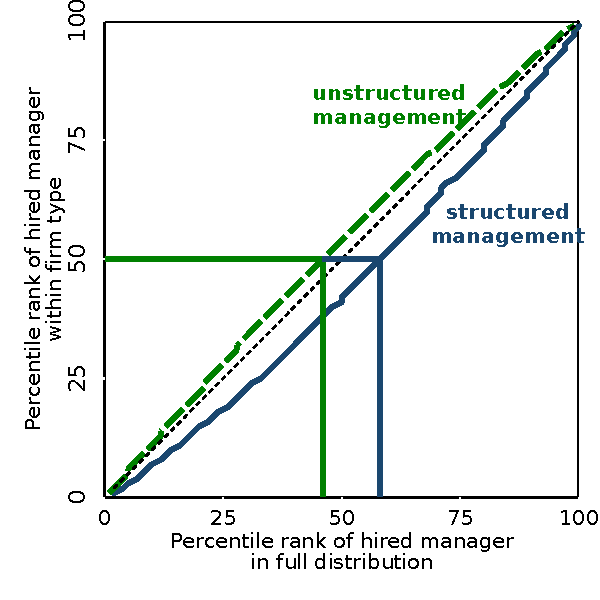
\includegraphics{./exhibits/fig_hiring_lorenz_mngr}
		\end{subfigure}
		\ \\
		\begin{subfigure}[b]{1\textwidth}
		  \centering
		   \caption{Production workers}
		  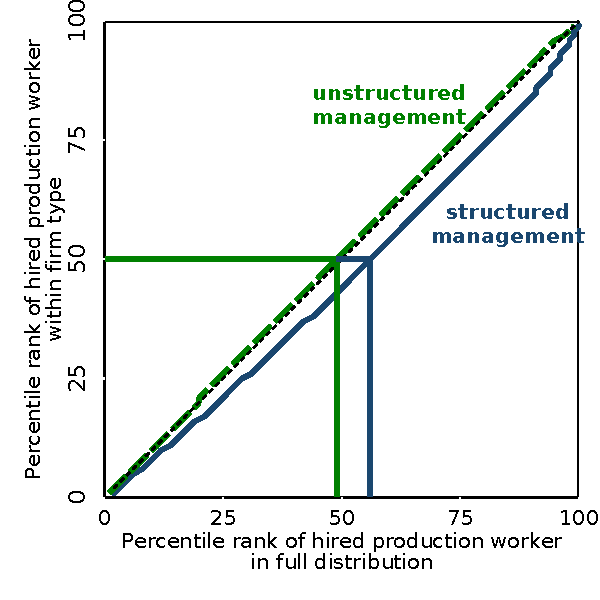
\includegraphics{./exhibits/fig_hiring_lorenz_labr}
		\end{subfigure}
		
	\end{figure}

% EXHIBIT: EMPLOYMENT SHARES BY WORKER QUALITY FOR STRUCTURED AD UNSTRUCTURED PROCESS FIRMS
\clearpage
	\begin{figure}[h]
		\centering
		\caption{Quality distribution of managers and production workers in continuing jobs}
		\label{fig:stayer_shares}
		\begin{subfigure}[b]{0.9\textwidth}
		  \centering
		  \caption{Managers}
		  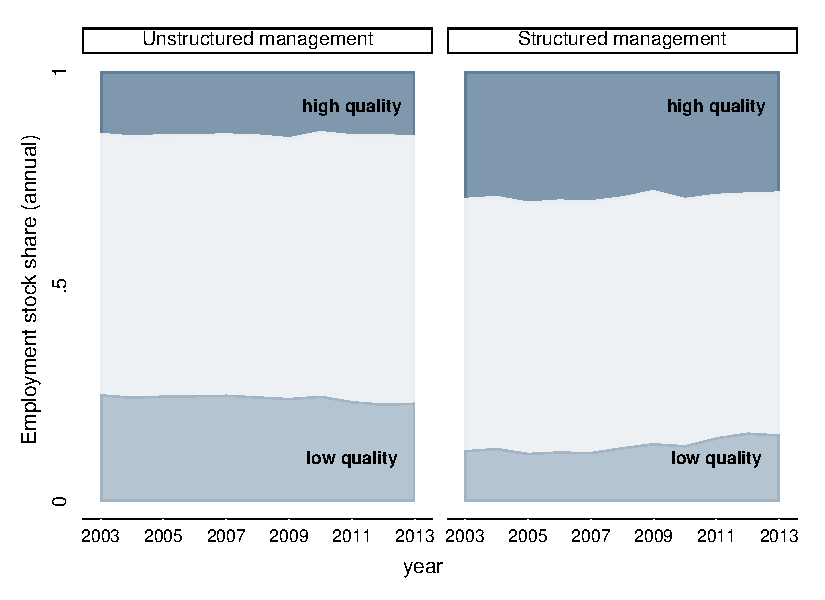
\includegraphics{./exhibits/fig_stayer_shares_mngr}\
		\end{subfigure}
		\ \\
		\begin{subfigure}[b]{0.9\textwidth}
		  \centering
		  \caption{Production workers}
		  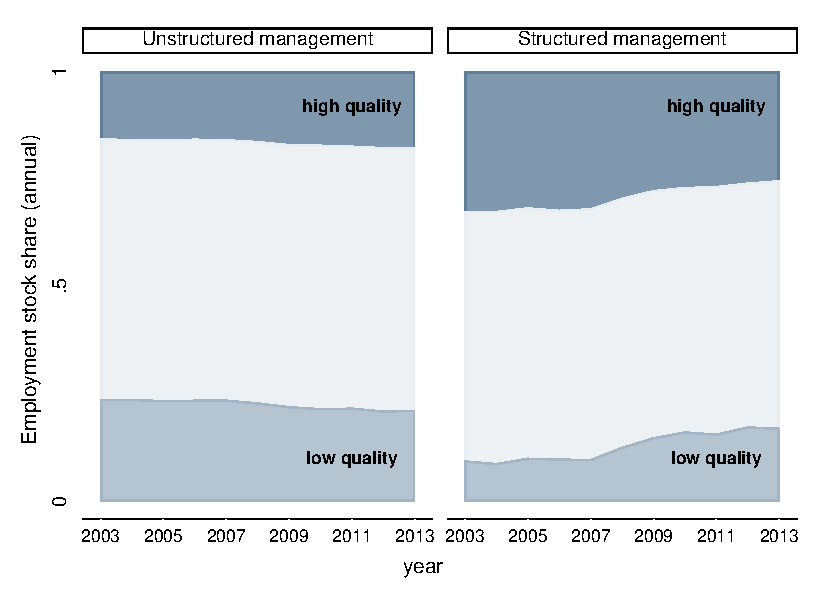
\includegraphics{./exhibits/fig_stayer_shares_labr}
		\end{subfigure}
	\end{figure}

% EXHIBIT: BIN SCATTERS OF FIRING RATES FOR MANAGERS AND PRODUCTION WORKERS
\clearpage
	\begin{figure}[ht]
		\centering
		\caption{Firing rates for managers and production workers by worker quality}
		\fbox{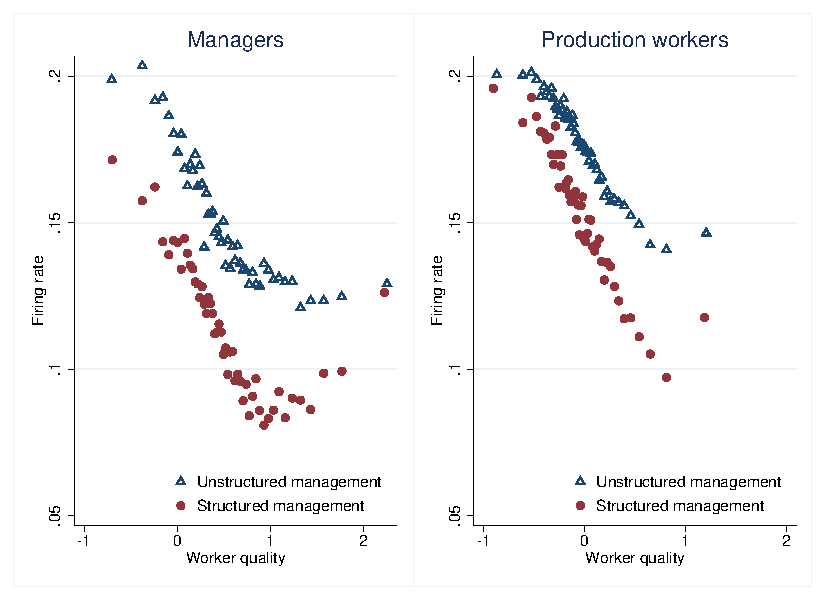
\includegraphics{./exhibits/fig_firing_binscatter}}
		\label{fig:firing_rate}
	\end{figure}
	
% EXHIBIT 5: TABLE 
\clearpage
\begin{landscape}
	\begin{table}
	\caption{Relationship between Worker and Management Quality} \label{tab:zpe_mgmt}
	\begin{center}
%	\scalebox{0.8}{
		\singlespace
		\small
		{
\begin{tabular}{l*{9}{c}}
\toprule
\textbf{Dependent variable:}  &\multicolumn{4}{c}{\textcolor{black}{z-(production worker quality)}}& & \multicolumn{4}{c}{\textcolor{black}{z-(manager quality)}} \\    \cline{2-5} \cline{7-10} 
				             &\multicolumn{1}{c}{(1)}&\multicolumn{1}{c}{(2)}&\multicolumn{1}{c}{(3)}&\multicolumn{1}{c}{(4)}&&\multicolumn{1}{c}{(5)}&\multicolumn{1}{c}{(6)}&\multicolumn{1}{c}{(7)}&\multicolumn{1}{c}{(8)}\\
                \midrule
 \textbf{Management indices} \\
z-people        &    0.100***&            &    0.098** &            &&    0.086***&            &    0.007   &            \\
                &  (0.036)   &            &  (0.042)   &            &&  (0.030)   &            &  (0.035)   &            \\
z-operations    &            &    0.074** &    0.004   &   -0.007   &&            &    0.143***&    0.137***&    0.130***\\
                &            &  (0.037)   &  (0.043)   &  (0.042)   &&            &  (0.033)   &  (0.040)   &  (0.040)   \\
                \\
\textbf{Individual practices} \\
z-talent mindset        &            &            &            &    0.091** &&            &            &            &    0.059*  \\
                &            &            &            &  (0.036)   &            &&            &            &  (0.031)   \\
z-performance culture        &            &            &            &    0.016   &&            &            &            &    0.008   \\
                &            &            &            &  (0.033)   &&            &            &            &  (0.032)   \\
z-talent capacity        &            &            &            &   -0.027   &&            &            &            &   -0.018   \\
                &            &            &            &  (0.033)   &&            &            &            &  (0.032)   \\
z-talent development        &            &            &            &    0.032   &&            &            &            &   -0.013   \\
                &            &            &            &  (0.041) &  &            &            &            &  (0.035)   \\
z-value proposition        &            &            &            &    0.016   &&            &            &            &   -0.015   \\
                &            &            &            &  (0.036)   &&            &            &            &  (0.037)   \\
z-retaining talent        &            &            &            &    0.017  & &            &            &            &   -0.009   \\
                &            &            &            &  (0.038)  & &            &            &            &  (0.033)   \\
Firm controls   &      Y   &      Y   &      Y   &      Y   &&      Y   &      Y   &      Y   &      Y   \\
Industry controls &      Y   &      Y   &      Y   &      Y   &&      Y   &      Y   &      Y   &      Y   \\
\midrule
\# Observations &\multicolumn{1}{c}{955}   &\multicolumn{1}{c}{955}   &\multicolumn{1}{c}{955}   &\multicolumn{1}{c}{955}   &&\multicolumn{1}{c}{955}  &\multicolumn{1}{c}{955}   &\multicolumn{1}{c}{955}   &\multicolumn{1}{c}{955}   \\
\# Firms        &      690   &      690   &      690   &      690   &&      690   &      690   &      690   &      690   \\
\(R^{2}\)       &    0.273   &    0.269   &    0.273   &    0.277   & &   0.353   &    0.360   &    0.360   &    0.362   \\
\bottomrule
\end{tabular}
}

%}
	\end{center}
\footnotesize{\textbf{Notes:} Results of linear regressions projecting plant-level averages of worker quality (estimated AKM worker effects) onto measures of management. 
In columns (1)--(4), the dependent variable is the average quality of production workers.
In columns (5)--(8), the dependent variable is the average quality of managers.
All models control for the log of employment, the year of observation (either 2008 or 2013), two-digit industry codes, the share of unionized workers, firm age, and whether the firm is multinational. 
In columns (1)--(3) and (5)--(7), the regressors of interest are the standardized measures of operations management and people management. In columns (4) and (8), the regressors of interest are the six subcomponents of the people-management measure. These measure the extent of structured management practices with respect to: (i) instilling a talent mindset; (ii) building a high-performance culture; (iii) making room for talent; (iv) developing talent; (v) creating a distinctive employee value proposition; (vi) retaining talent. For details of these different measures, see \citet{bloom_qje2007} and \citet{wms_jeea}.}
	\end{table}
\end{landscape}





























	

	% ------------------------------ Appendix --------------------------
\clearpage
\begin{center}
{\bf Appendix for Cornwell, Schmutte, and Scur ``\mytitle,'' \today}
\end{center}


% \noindent The full manuscript is available at 
% \href{http://www.kurtlavetti.com/CDEM_vc.pdf}{http://www.kurtlavetti.com/CDEM\_vc.pdf}. Please contact the authors at \href{mailto:lavetti.1@osu.edu}{lavetti.1@osu.edu} or \href{mailto:schmutte@uga.edu}{schmutte@uga.edu} with comments or for additional information.

	\appendix 
	% \singlespacing
	\setcounter{table}{0}
	\setcounter{figure}{0}
	\pagenumbering{arabic}\renewcommand{\thepage}{App.~\arabic{page}}
	\renewcommand\thetable{\Alph{section}.\arabic{table}}
	\renewcommand\thefigure{\Alph{section}.\arabic{figure}}
	\renewcommand\theequation{\Alph{section}.\arabic{equation}}
	\input{./AERI-appendix}

\end{document}

